\chapter{高频功率放大器}

\section{概述}

功率放大电路是一种以输出较大功率为目的的放大电路。

功能:将直流功率转换为交流信号功率。

主要指标:输出功率与效率。

工作状态:丙类大信号的非线性状态 (非线性失真)。

分析方法:折线近似分析法 (大信号)。

\subsection{高频功率放大器与低频功率放大器的异同}

相同点:要求输出功率大,效率高。

不同点:低频功率放大器相对频带宽;高频功率放大器相对频带很窄,可以用调谐回路作负载,能工作于丙类。

\subsection{功率放大电路的主要特点}

输入为大信号、输出功率尽可能大、管子工作在接近极限状态、效率要高、非线性失真要小、BJT 散热要好。

属于非线性工作状态;基极偏置为负值,$\theta_c < 90^\circ$,电流脉冲是尖顶余弦脉冲;负载是 LC 谐振回路。

要解决的问题:提高输出功率、提高效率、管子的保护、减小失真(线性度)。

\section{谐振功率放大器的工作原理 \textcolor{red}{$\bigstar$}}

\subsection{获得高效率所需要的条件}

小信号谐振放大器与丙类谐振功率放大器的区别之处在于:工作状态分别为小信号甲类与大信号丙类。因此,采用负电源作基极偏置。

\subsection{功率关系}

电路正常工作(丙类、谐振)时,外部电路关系式:

\begin{equation}
    P_= = V_{CC} I_{C0}, \quad P_o = \frac{1}{2} V_{cm} I_{cm1} = \frac{V_{cm}^2}{2R_p} = \frac{1}{2} I_{cm}^2 R_p
\end{equation}

其中 $P_=$ 为直流输入功率, $P_o$ 为交流输出功率,$R_p$ 为负载阻抗。 $P_= = P_o + P_c $, $P_c$ 为集电极直流功耗。

集电极效率为:

\begin{equation}
    \eta_c = \frac{P_o}{P_=} = \frac{\dfrac{1}{2} V_{cm} I_{cm1}}{V_{CC} I_{C0}} = \frac{1}{2} \xi g_1(\theta_c)
\end{equation}

其中,$\xi = \dfrac{V_{cm}}{V_{CC}}$ 为集电极电压利用系数,$g_1(\theta_c) = \dfrac{I_{cm1}}{I_{C0}}$ 为波形系数。半流通角 $\theta_c$ 通常取 $70^\circ$。

\section{晶体管谐振功率放大器的折线近似分析法 \textcolor{red}{$\bigstar$}}

\subsection{晶体管特性曲线的理想化及其解析式}

\begin{figure}[htbp]
    \centering
    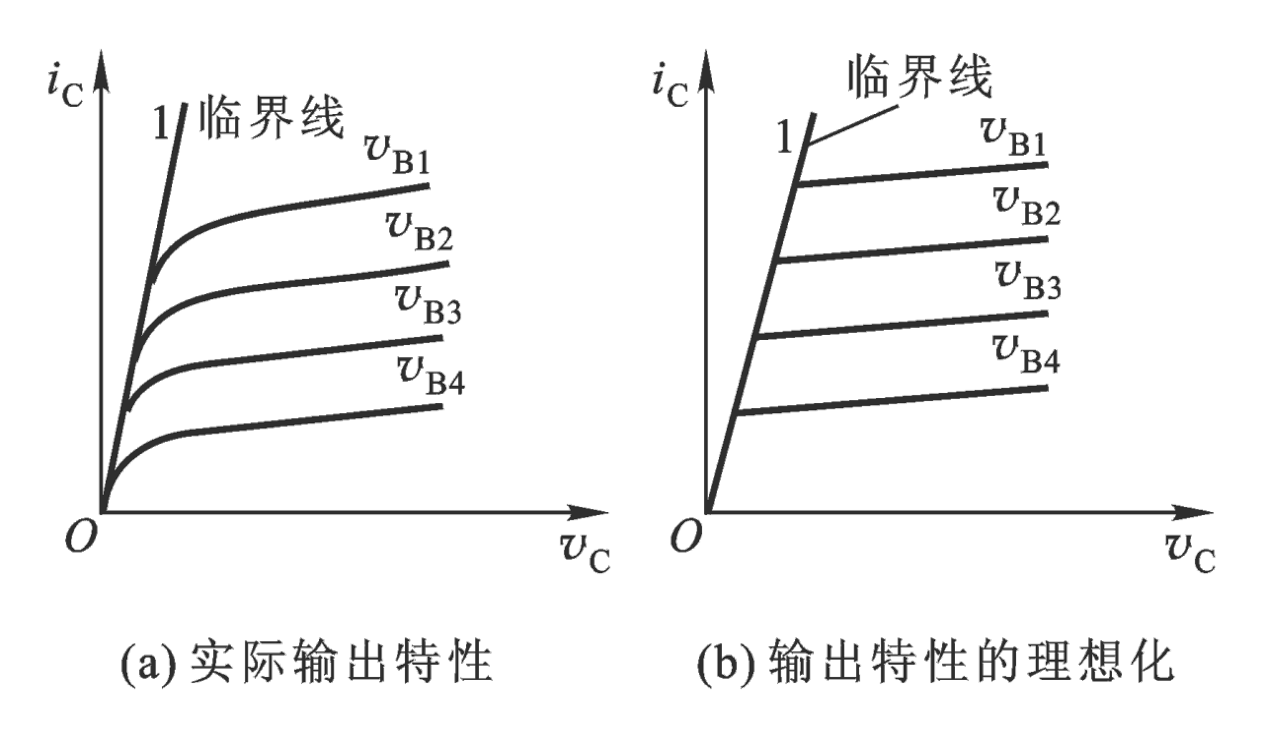
\includegraphics[scale=0.5]{image/Picture2.png}
    \caption{晶体管的输出特性}
\end{figure}

临界线方程为:

\begin{equation}
    i_C = g_{cr} v_C
\end{equation}

\begin{figure}[htbp]
    \centering
    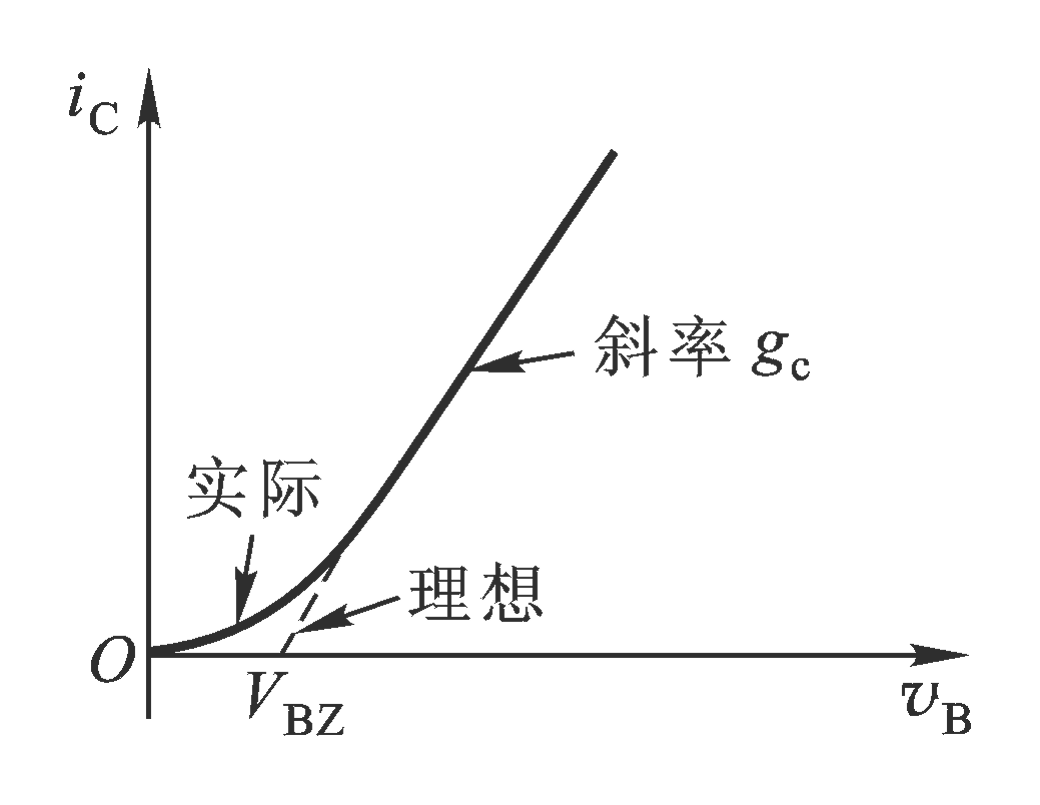
\includegraphics[scale=0.3]{image/Picture3.png}
    \caption{晶体管静态转移特性}
\end{figure}

晶体管静态转移特性理想化:

\begin{equation}
    i_C = g_c (v_{BE} - V_{BZ}), (v_{BE} > V_{BZ}) 
\end{equation}

\subsection{集电极余弦电流脉冲的分解}

用折线法对集电极余弦电流脉冲进行分解得出:

\begin{equation}
\begin{aligned}
    i_{C \text{max}}  &= g_c V_{bm} (1 - \cos{\theta_c}) \\
    \cos{\theta_c} &= \frac{V_{BB} + V_{BZ}}{V_{bm}} \\
    I_{C0}  &= i_{C \text{max}} \alpha_0(\theta_c) \\
    I_{cm1} &= i_{C \text{max}} \alpha_1(\theta_c) \\
    I_{cmn} &= i_{C \text{max}} \alpha_n(\theta_c) 
\end{aligned}
\end{equation}

\subsection{高频功率放大器的动态特性与负载特性}

高频放大器的工作状态是由负载阻抗 $R_p$、激励电压 $v_b$、供电电压 $V_{CC}$、$V_{BB}$ 共 4 个参量决定的。

高频功放的动态特性表达式 (直线):

\begin{equation}
    i_C = g_d (v_c - V_o) 
    = - g_c \frac{V_{bm}}{V_{cm}} \left[ v_c - (V_{CC} - V_{cm} \cos{\theta_C}) \right]
\end{equation}

负载线的虚拟 Q 点坐标为:$[V_{CC}, - g_c(V_{BB} + V_{BZ})]$。负载线的延长线必过 Q 点。

\begin{figure}[htbp]
    \centering
    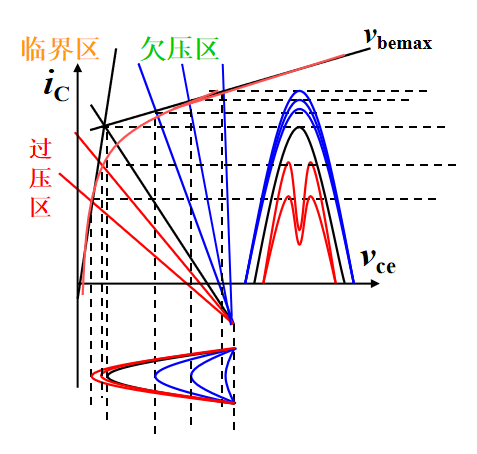
\includegraphics[scale=0.7]{image/Picture4.png}
    \caption{高频功放的动态特性}
\end{figure}

\begin{figure}[htbp]
    \centering
    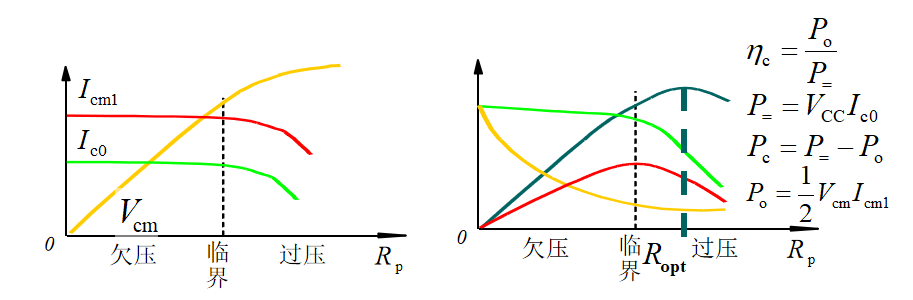
\includegraphics[scale=0.8]{image/Picture5.png}
    \caption{高频功放的负载特性}
\end{figure}

欠压、过压、临界三种工作状态的特点:

① 欠压:恒流,$V_{cm}$变化,$P_o$较小,$\eta_c$低,$P_c$较大;晶体管基极调幅需采用这种工作状态。

② 过压:恒压,$I_{cm1}$变化,$P_o$较小,$\eta_c$可达最高;用于中间放大级、集电极调幅级。

③ 临界:$P_o$最大,$\eta_c$较高;用于发射机末级,是最佳工作状态。

临界状态时,记临界线斜率为 $g_{cr}$,$v_C$ 的最小值 $v_{C_{\text{min}}} = V_{C_{\text{sat}}} = \dfrac{i_{C_{\text{max}}}}{g_{cr}}$,即集电极饱和电压。此时一般使用 $V_{cm} = V_{CC} - V_{C_{\text{sat}}}$ 来求 $V_{cm}$。

\subsection{各极电压对工作状态的影响}

调整工作状态的几种方法:

改变集电极负载 $R_p$、改变供电电压 $V_{CC}$、改变偏压 $V_{BB}$、改变激励 $V_{bm}$。

(1) 仅 $R_p$ 由小到大变化时,放大器的工作状态:欠压 $\rightarrow$ 临界 $\rightarrow$ 过压。

(2) 仅 $V_{CC}$ 由小到大变化时,放大器的工作状态:过压 $\rightarrow$ 临界 $\rightarrow$ 欠压。

(3) 仅 $V_{bm}$ 由小到大变化时,放大器的工作状态:欠压 $\rightarrow$ 临界 $\rightarrow$ 过压。

(4) 仅 $V_{BB}$ 由小到大变化时,放大器的工作状态:过压 $\rightarrow$ 临界 $\rightarrow$ 欠压。

过压状态下,$V_{bm}$ 和 $R_p$ 有一个改变时,$V_{cm}$ 基本不变。

欠压状态下,$V_{bm}$ 和 $V_{BB}$ 均不改变时,$I_{C0}$ 和 $I_{cm1}$ 基本不变。

\subsection{工作状态的计算举例}

(1) 以临界状态为例,首先要求得集电极电流脉冲的两个主要参量集电极电流脉冲幅值 $i_{C_{\text{max}}}$ 和导通角 $\theta_c$。

\begin{equation}
\begin{aligned}
    i_{C \text{max}}  &= g_c V_{bm} (1 - \cos{\theta_c}) \\
    \cos{\theta_c} &= \frac{V_{BB} + V_{BZ}}{V_{bm}}
\end{aligned}
\end{equation}

(2) 电流余弦脉冲的各谐波分量系数 $\alpha_0(\theta_c) \dots \alpha_n(\theta_c)$ 可查表求得,并求得个分量的实际值。

\begin{equation}
\begin{aligned}
    I_{C0}  &= i_{C \text{max}} \alpha_0(\theta_c) \\
    I_{cm1} &= i_{C \text{max}} \alpha_1(\theta_c) \\
    I_{cmn} &= i_{C \text{max}} \alpha_n(\theta_c) 
\end{aligned}
\end{equation}

(3) 求解谐振功率放大器的功率和效率。其直流功率、交流输出功率、集电极效率分别为:

\begin{equation}
\begin{aligned}
    P_= &= V_{CC} I_{C0} \\
    P_o &= \frac{1}{2} V_{cm} I_{cm1} = \frac{V_{cm}^2}{2R_p} = \frac{1}{2} I_{cm}^2 R_p \\
    \eta_c &= \frac{P_o}{P_=} = \frac{\dfrac{1}{2} V_{cm} I_{cm1}}{V_{CC} I_{C0}} = \frac{1}{2} \xi g_1(\theta_c)
\end{aligned}
\end{equation}

(4) 最佳负载电阻 (在临界工作时,$\xi$ 接近于 $1$,可直接取 $1$):

\begin{equation}
    R_p = \frac{(\xi V_{CC})^2}{2 P_o}
\end{equation}


